\chapter{Umsetzung}
	Nachdem im vorherigen Kapitel die technischen Grundlagen erläutert wurden, wird nun auf die Umsetzung eingegangen. Es wird mit der Umgesetzten Architektur begonnen, um einen groben Überblick über die einzelnen Komponenten zu bekommen. Anschließend wird genauer auf zwei wesentliche Teile eingegangen:

	\paragraph{Datenhaltung und Anbindung an eine Datenbank}
		In diesem Abschnitt wird die Datenhaltung auf dem Handy beschrieben. Dabei wird auf zwei unterschiedliche Methoden eingegangen, die bei der Umsetzung zum Einsatz kamen. In dem ersten Abschnitt wird auf die Datenbankanbindung an den Server eingegangen. Besonders wird hier auf die verschiedenen Tabellen der Datenbank Bezug genommen und das allgemeine vorgehen beschrieben, Daten vom Server zu Laden und dort zu Speichern. Im Zweiten wird mehr auf die lokale Speicherung und Datenhaltung Bezug genommen und die verschiedenen Verfahren erläutert.

	\paragraph{Bestandteile der App}
		In diesem Abschnitt wird sich mit den generellem Aufbau der App befasst und teilt sich in zwei weitere Teile auf. in Teil eins wir auf die Benutzerschnittstelle eingegangen und die Benutzeroberfläche von NoRPG erklärt. Im zweiten Teil wird auf weitere wichtige Bestandteile der App eingegangen, darunter wichtige Klassen, welche für die App unverzichtbar sind.

	\section{Architektur}
		Die Architektur entspricht dem Model View Controller Prinzip, bei dem es eine zentrale Schnittstelle einen Controller gibt. In diesem Fall ist das die Klasse „GameControl.cs”, welche den Datenzugriff  zwischen App und Server regelt und innerhalb der App alle wichtigen Abhängigkeiten widerspiegelt. Diese Klasse ist darüber hinaus auch die zentrale Stelle zum speichern und laden von Daten. In Abbildung \ref{architecture} ist die Architektur grafisch dargestellt.

		\begin{figure}[htbp]
			\centering 
			\label{architecture}
			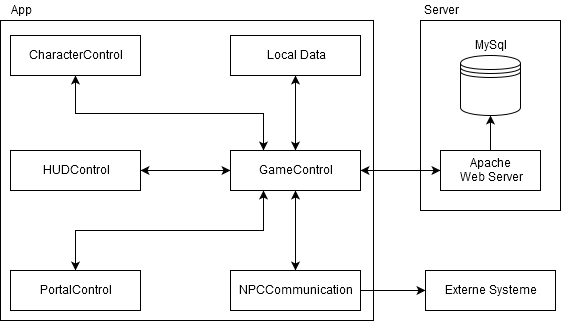
\includegraphics[width=13cm]{pics/archtecture.png}
			\caption{Softwarearchitektur}
		\end{figure}	

		Darauf ist zu erkennen, dass die Klasse „GameController.cs” eine zentrale Rolle in der App spielt und im Mittelpunkt steht. Auf dem Server steht eine MySql Datenbank bereit, welche sich um die persistente Datenhaltung kümmert. Neben GameController.cs” ist der NPCCommunicationController die einzige Klasse, welche außerhalb der eigentlichen Applikation kommuniziert. Das tut sie mit einem \ac{JSON} Parser Plugin, welches beim auslesen der \ac{JSON} Dateien hilft (siehe Kapitel \ref{npctext}).	

	\section{Datenhaltung und Anbindung an eine Datenbank}
		In diesem Kapitel wird die Datenhaltung auf dem Handy und dem Server erläutert. Begonnen wird dabei mit der Beschreibung der Datenhaltung auf dem Handy. Dabei wird auf verschiedene Aspekte der Speicherung eingegangen.
		
\subsection{Anbindung an einen Server}
			Zum Senden der Daten der Registrierung wird das Skript „SendDataToServer.cs” genutzt. In diesem werden die Daten der Registrierung zwischengespeichert und am Ende an den Server gesendet. Dazu wird die Methode „SendRegister()” genutzt. In dieser wird die Methode „RegisterUser()” als Coroutine gestartet. Dazu werden zehn Parameter übergeben, der Username, die Email, das Passwort, der Vorname, der Nachname, das Geburtsdatum, das Geschlecht, der Herkunftsstaat, die native Sprache und der gewählte Charakter. Bei einer Coroutine handelt es sich um einen Thread, welcher beliebig gestartet, pausiert und beendet werden kann.

			Innerhalb dieser Methode wird zu Beginn ein Hash erstellt, welcher am Server genutzt wird, um zu überprüfen, ob die Anfrage gültig ist. Dieser besteht dabei aus teilen der Eingabe und einem zusätzlichen geheimen Schlüssel, welchem nur der App und dem Server bekannt sind. Dadurch wird die Sicherheit gesteigert und es wird Angreifern erschwert unberechtigte Zugriffe auf die Datenbank zu tätigen. Bei dm Hash handelt es sich dabei um die MD5 verschlüsselten Eingabedaten. Dadurch ist es fast nicht möglich, einen Validen Hash zu bilden, ohne diese Daten zu kennen.

			Nachdem der Hash erstellt wurde, werden alle Parameter in Form einer URL aneinander gehängt. Anschließend wird die URL an ein WWW Objekt übergeben und solange gewartet, bis es eine Antwort gibt. Sofern es keinen Fehler gab, wird ein Text ausgegeben, welche vom Server gesendet wird, andernfalls eine Fehlermeldung.

			\begin{scriptsize}
				\lstset{
					float,
					caption=Skript SendDataToServer.cs, 
					language=[Sharp]C, 
					frame=single,  
					showstringspaces=false, 
					showspaces=false, 
					numbers=left, 
					captionpos=b, 
					belowcaptionskip=4pt,
					basicstyle=\ttfamily
				} 
				\begin{lstlisting}[label=lst:c_SendDataToServer]
public class SendDataToServer : MonoBehaviour {
  private static string secretKey = "*****";
  public static string registerURL = "http://norpg.it.dh-karlsruhe.de/register.php?";
  public static string loginURL = "http://norpg.it.dh-karlsruhe.de/login.php?";

  [...]
	
  private void SendRegister() {
    StartCoroutine(RegisterUser(userText, emailText, MD5Test.Md5Sum(passwordText), 
    firstnameText, lastnameText, birthdayText, genderText, 
    countryText, native_languageText, selected_characterText));
  }
	
  IEnumerator RegisterUser(string user, string email, string password, string firstname, 
    string lastname, string birthday, string gender, string country, 
    string native_language, string selected_character) {
	
    string hash = MD5Test.Md5Sum(user + email + password 
    + firstname + country 
    + selected_character + secretKey);

    string post_url = registerURL
    + "user=" + WWW.EscapeURL(user)
    + "&email=" + WWW.EscapeURL(email)
    + "&password=" + WWW.EscapeURL(password)
    + "&firstname=" + WWW.EscapeURL(firstname)
    + "&lastname=" + WWW.EscapeURL(lastname)
    + "&birthday=" + WWW.EscapeURL(birthday)
    + "&gender=" + WWW.EscapeURL(gender)
    + "&country=" + WWW.EscapeURL(country)
    + "&native_language=" + WWW.EscapeURL(native_language)
    + "&selected_character=" + WWW.EscapeURL(selected_character)
    + "&hash=" + hash;
    
    WWW hs_post = new WWW(post_url);
    yield return hs_post;

    if (hs_post.error != null) {
      print("There was an error posting the high score: " + hs_post.error);
    } else {
      status.text = hs_post.text;
    }
  }
}
				\end{lstlisting}
			\end{scriptsize}

			Auf dem Server läuft für die Datenannahme das PHP Skript „register.php”. Dieses nimmt die Daten aus der URL entgegen und speichert diese zunächst in Variablen ab. Anschließend wird auch in diesem Skript ein Hash gebildet und anschließend mit dem Mitgesendetem abgeglichen. Sollte es hier einen Fehler geben, sendet der Server einen Error zurück, wenn die Hashes identisch sind, wird eine Verbindung zu der Datenbank aufgebaut und ein Eintrag in der accounts Tabelle erstellt. Anschließend wird eine erfolgreich Meldung an den Client gesendet.

			Für den Login innerhalb der App wird identisch vorgegangen. Dabei wird jedoch ein Datensatz in die Datenbank geschrieben, sondern nur gelesen. Des weiteren wird der Hash aus weniger Werten gebildet, da nur der Username und das verschlüsselte Passwort übermittelt werden.
			
			Auf dem Server läuft eine MySQL Datenbank. Diese sorgt für eine permanente Datenhaltung und die Synchronisation zwischen den Clients. Die Datenbank besteht dabei aus den  Tabellen „accounts” und „player\_data”. In „accounts” sind alle Informationen zu einem User hinterlegt, darunter auch die Daten für den Login. In der Tabelle „player\_data” wird der Fortschritt von jedem Spieler gespeichert, damit dieser von jedem Gerät aus erreichbar ist.

		\subsection{Datenhaltung auf dem Handy}
		
			Die Daten auf dem Handy werden im \ac{JSON}-File Format gespeichert. Es gibt zwei verschiedene \ac{JSON} Dateien in der App, eines für die Standards, welches vom Server geladen wird, und eines für die Texte der \acp{NPC}. Beide Dateien werden unterschiedlich ausgelesen und genutzt. Zuerst wird auf die Standards eingegangen und anschließend auf die Verarbeitung der Datei mit Texten der \acp{NPC}. 

			\subsubsection{Standards \ac{JSON}}
				Die \ac{JSON} für die Standards ist ein wichtiger Bestandteil des Spieles. In dieser Datei befinden sich alle wichtigen Infos zu den Standards und deren dazugehörigen Spiele. Diese Datei liegt Zentral auf einem Server und kann dort gewartet und gepflegt werden. Dadurch ist es möglich, zusätzliche Standards und Spiele einzufügen, ohne das der Nutzer die App aktualisieren muss. Nun wird der grobe Ablauf, gefolgt von einer detaillierten Beschreibung, erklärt und beschrieben.

				Damit der Nutzer die aktuelle Datei zur Verfügung hat, versucht das Spiel eine zu Beginn eine Verbindung zu dem Server aufzubauen. Gelingt dies, wird die Datei von Server geladen und auf dem Handy gespeichert. Nachdem die Datei gespeichert wurde, wird sie in das Spiel geladen. Dazu wird aus dem \ac{JSON} eine Liste erstellt, welche überall im Spiel nutzbar ist.

				Für das Laden und verarbeiten sind fünf Klassen verantwortlich. Im Folgenden wird nur detailliert auf die Klasse „WebJSONConfigReader” eingegangen. Die anderen Klassen sind im Anhang abgebildet und werden nur erwähnt.

				Die Klasse „MappingStandardsToCourses” ist die Datenhaltungsklasse. In dieser ist die Struktur der einzelnen Objekte geregelt. In der Klasse „MappingStandardsToCoursesBean” spiegelt die Struktur der \ac{JSON}-Datei wieder. 

				Der „WebJSONConfigReader” wird in der Klasse „LoadingScreen” genutzt. Dort wird eine Instanz dieser Klasse erzeugt und es wird die Methode „LoadSettings” ausgeführt und in der Variable „Settings” gespeichert. Diese Methode ist in Listing \ref{lst:methode3} zu sehen.

			\begin{scriptsize}
				\lstset{
					float,
					caption=Methode LoadSettings, 
					language=[Sharp]C, 
					frame=single,  
					showstringspaces=false, 
					showspaces=false, 
					numbers=left, 
					captionpos=b, 
					belowcaptionskip=4pt,
					basicstyle=\ttfamily
				} 
				\begin{lstlisting}[label=lst:methode3]
public MappingStandardsToCourses LoadSettings() {
  WWW www = new WWW(settingsURL);
  while (!www.isDone) { }
  string json;
  string LocalFilePath = Application.persistentDataPath + "/v1.json";
	
  if (string.IsNullOrEmpty(www.error)) {
    json = www.text;
    File.WriteAllText(LocalFilePath, json);
  } else if (File.Exists(LocalFilePath)) {
    json = File.ReadAllText(LocalFilePath);
  } else {
    json = "";                
    File.WriteAllText(LocalFilePath, json);
  }

  MappingStandardsToCoursesBean settingsBean = 
    MappingStandardsToCoursesBean.CreateFromJSON(json);
  
  string json2 = JsonUtility.ToJson(settingsBean);	
  List<Classes> classes = new List<Classes>();
  foreach (var classe in settingsBean.classes) {
    List<Courses> courses = new List<Courses>();
    foreach (var course in classe.courses) {
      List<Standards> standards = new List<Standards>();
      foreach (var standard in course.standards) {
        List<Games> games = new List<Games>();
        List<string> vor = new List<string>();
        List<string> nach = new List<string>();
        foreach (var game in standard.games) {
          games.Add(new Games(game.id, game.name, game.url));
        }
        foreach (var vorbedingung in standard.vorbedingungen) {
          vor.Add(vorbedingung);
        }
        foreach (var nachbedingung in standard.nachbedingungen) {
          nach.Add(nachbedingung);
        }
        Games[] g = games.ToArray();
        string[] v = vor.ToArray();
        string[] n = nach.ToArray();
        standards.Add(new Standards(standard.name, v, n, g));
      }
      Standards[] s = standards.ToArray();
      courses.Add(new Courses(course.name, s));
    }
    Courses[] c = courses.ToArray();
    classes.Add(new Classes(classe.name, c));
  }
  Classes[] cla = classes.ToArray();
  return new MappingStandardsToCourses(cla);
}
				\end{lstlisting}
			\end{scriptsize}

				In dieser wird zu Beginn ein neues WWW Objekt erstellt. Dieses baut eine Verbindung zum Server auf. Anschließend wird in Zeile 9 überprüft, ob es zu einem Fehler beim Verbindungsaufbau gekommen ist. Wenn es zu keinem Fehler gekommen ist, wird der Inhalt des WWW Objekts in eine Datei geschrieben und gespeichert. Für den Fall das ein Fehler aufgetreten ist und das WWW Objekt keine Verbindung zum Server aufgebaut werden kann, wird geprüft ob bereits eine ältere Datei vorhanden ist, wenn ja, wird der Text aus dieser Datei zum Erzeugen des Objektes genutzt. Anschließend wird in Zeile 19 aus dem Text eine \ac{JSON} Struktur erzeugt. Aus dieser wird anschließend in mehreren Schritten ein mehrdimensionaler Array erzeugt und zurückgegeben.

			\section{Benutzerschnittstelle}
		In diesem Abschnitt dieses Kapitels wird auf die Umsetzung der Benutzerschnittstelle eingegangen. Wie schon bereits im \ac{SRS} erwähnt handelt es sich bei der Benutzerschnittstelle um die grafische Oberfläche der Anwendung. Dafür wird zunächst auf die Umsetzung der verschiedenen \ac{UI} Elemente eingegangen sowie relevante Funktionalitäten beschrieben. Abschließend wird die Evaluation des Usability Tests behandelt. 

		\subsection{Benutzeroberfläche}	
			Die Implementierung der Benutzeroberfläche ist von Anfang der Umsetzungsphase bis zum Ende ein kontinuierlicher, iterativer und wichtiger Entwicklungsprozess. Es beginnt mit einer ganz simplen Steuerung zum Testen von Funktionen bis zum Perfektionieren aller benötigter User Interface Elemente. Als erstes werden die Startbildschirme und der Registrierungsprozess behandelt. 

			\subsubsection{Startbildschirm und Registrierung}
				Das aller erste, was der Spieler von NoRPG sieht und womit er interagieren darf, ist der Startbildschirm. Dieser ist besonders wichtig, da hier die ersten Eindrücke schon gesammelt werden. Bei dem Startbildschirm wird zwischen zwei Varianten unterschieden. In der ersten Variante startet der Spieler NoRPG das erste mal oder ist nicht mit seinem Account angemeldet. In der zweiten Variante ist der Benutzer schon angemeldet. Diese beide Varianten sind in der Grafik \ref{startScreenUI} dargestellt.

				\begin{figure}[htbp]
					\centering 
					\label{startScreenUI}
					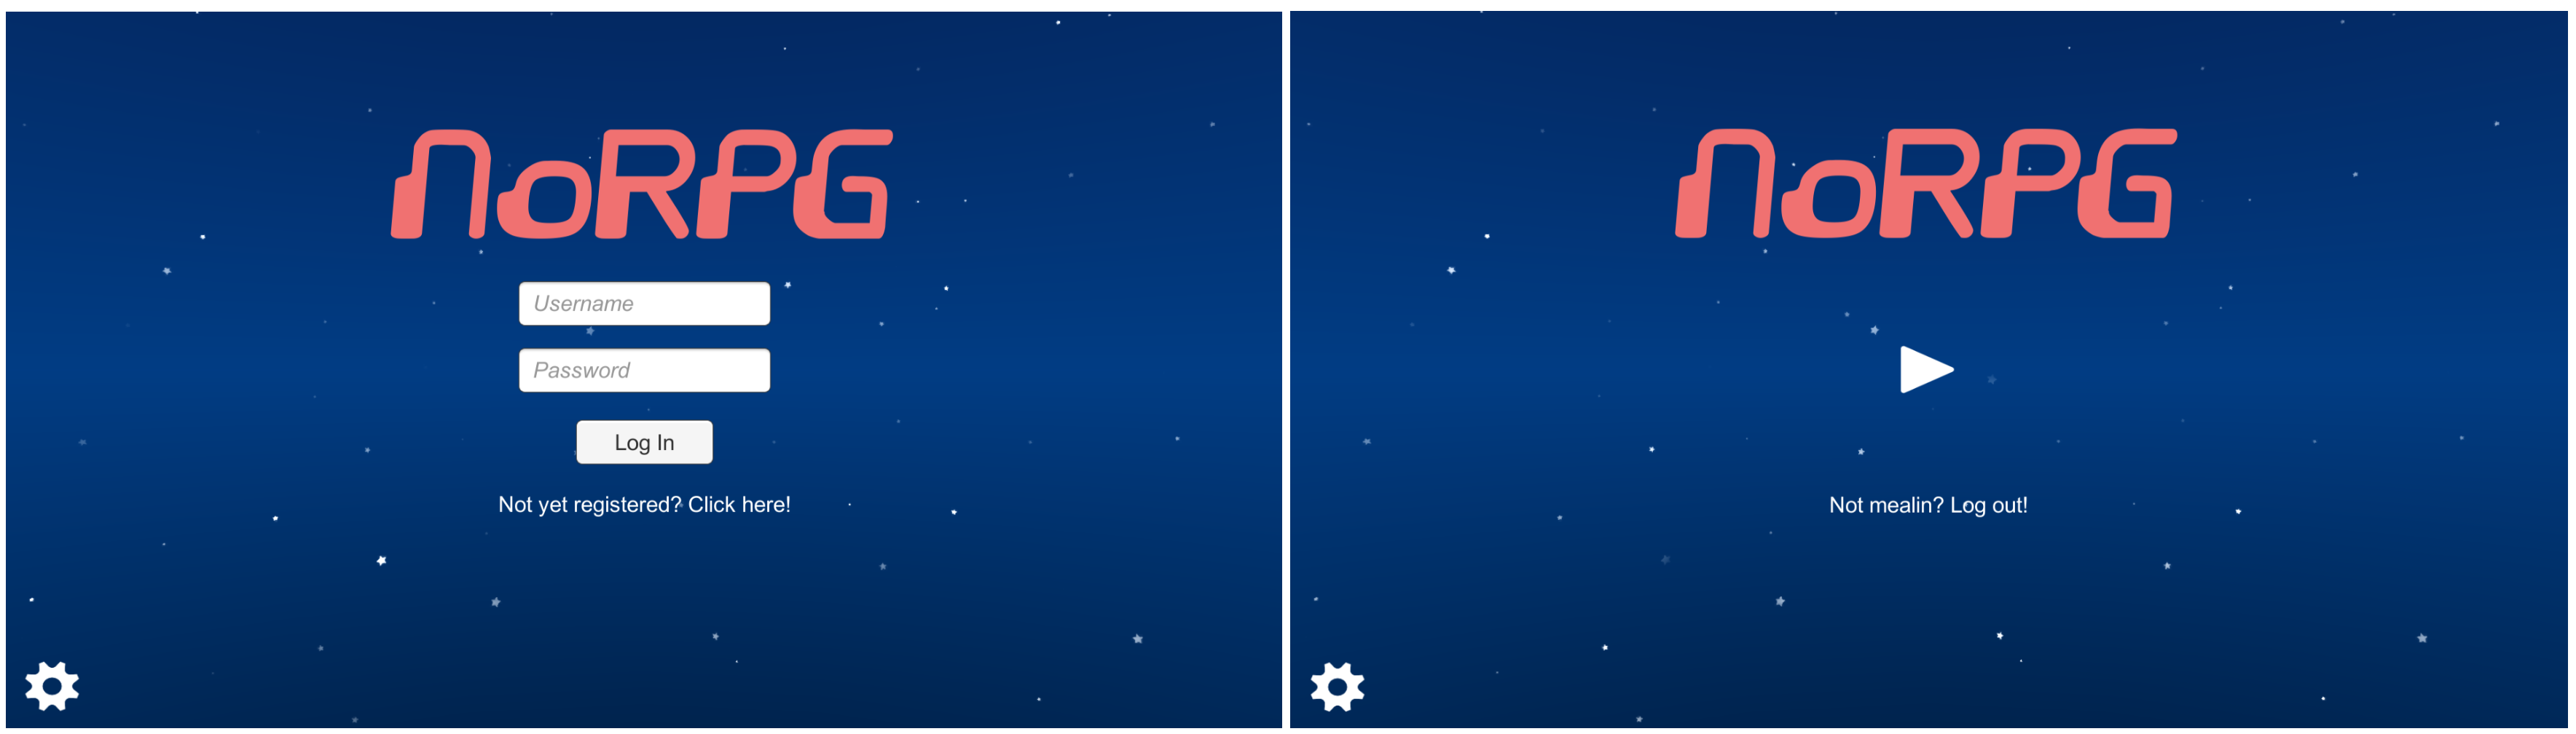
\includegraphics[width=\textwidth]{pics/startbildschirmeScreen.png}
					\caption{User Interface: Startbildschirm}
				\end{figure}

				Beide Varianten ähneln sich nicht nur im aussehen sondern auch in der Implementierung. Die Startbildschirme wurden nach dem Gestaltungsprinzip Figure/Ground entworfen und umgesetzt. Figure/Ground unterteilt die Wahrnehmung visueller Informationen in Figure (Vordergrund) und Ground (Hintergrund). Dabei liegt der Fokus auf dem Vordergrund. Das Design und Aussehen der Komponenten ist dabei Clean und Simple, zu Deutsch sauber und einfach. Dieter Rams beschreibt in seinem Buch "Weniger, aber besser / Less but better" \cite{ramsDesign}, dass einfaches Design nicht über die Subtraktion von Dingen von einem Design handelt, sondern die Gesamteffektivität des Designs zu verbessern. Elemente in der Benutzeroberfläche haben so wenig Text und Farbe wie notwendig und werden, falls möglich, nur mit Symbole abgebildet. Dabei wird ein intuitives Design verwendet, welches die Spieler wahrscheinlich aus anderen Spielen schon kennen und nicht neu lernen müssen.

				Der Vordergrund von beiden Varianten ist in zwei Abschnitte unterteilt. Der erste Abschnitt ist in der Mitte des Bildschirm positioniert und bindet die Aufmerksamkeit des Spielers. In der ersten Variante besteht dieser aus zwei Eingabefelder für die Benutzerdaten, dem Log-In Button und einem Textfeld, um sich zu registrieren. In der zweiten Variante allerdings besteht dieser Abschnitt nur aus einem Button zum Starten des Spieles und einem Textfeld für die Abmeldung. Der zweite Abschnitt ist an der unteren Seite des Bildes positioniert und besteht aus einem Button für die Einstellungen. Dabei öffnet sich kein Fenster, sondern werden Symbole für die Einstellungsmöglichkeiten ein- und ausgeblendet.

				Der Hintergrund setzt sich aus dem Logo und einem Sternenhimmel zusammen. Diese Hintergrundelemente sind 3D-Elemente, welche in der Spielwelt angebracht sind und durch eine Kamera aufgezeichnet werden. Neben diesen Hintergrundelementen gibt es ein weiteres Element, welches erst durch die Betätigung des Log-In Buttons auftaucht. Es handelt sich um ein drehendes Icon, dass den Ladeprozess darstellt und somit dem Spieler ein Feedback gibt. Der Hintergrund ist sehr schlicht aber farbenfroh gestaltet. Zudem sind die Sterne am Himmel animiert, welches einen besonders positiven Eindruck hinterlassen soll.

				Die Startbildschirme sind mit dem Standard Render-Modus Screen Space - Overlay umgesetzt worden. Dieser Modus unterstützt das Gestaltungsprinzip Figure/Ground, indem die \ac{UI} Elemente vor den Hintergrund gerendert werden. Fernerhin kann der Spieler sich innerhalb des Startbildschirm nicht bewegen oder andere Interaktionen ausführen, sodass ein anderer Render-Modus notwendig wäre.

				Auf Grund der Tatsache das es zwei Startbildschirme gibt, muss bevor der anzuzeigende Startbildschirm angezeigt wird eine Überprüfung stattfinden. Die aller erste Szene die in NoRPG geladen wird, ist eine nahezu leere Szene, die nur aus dem Hintergrund, einem kleinen Textfeld und einem Skript besteht. Diese Szene ist deshalb so minimalistisch gestaltet, damit das Laden und somit das Ausführen des Skriptes sehr schnell durchgeführt werden kann, so dass der Spieler im besten Fall diese Szene erst gar nicht sieht und bemerkt. Das Skript prüft, ob die in Kapitel 5.1 beschriebene lokale Datei, mit den Informationen über den Spielstand des Spielers, vorhanden und vollständig ist. Ist dies der Fall, kann davon ausgegangen werden, dass der Spieler angemeldet ist und die zweite Variante des Startbildschirmes wird geladen. Der Hintergrund ist notwendig, falls das Laden länger braucht der Spieler keinen weißen beziehungsweise leeren Hintergrund sieht. Das Textfeld in dieser Szene ist angebracht, damit der Spieler im Fehlerfall informiert wird.

				Die nächste Benutzeroberfläche, die behandelt wird, ist die Registrierung. Ein Teil des Registrierungsprozesses ist in Abbildung \ref{registerUI} abgebildet.

				\begin{figure}[htbp]
					\centering 
					\label{registerUI}
					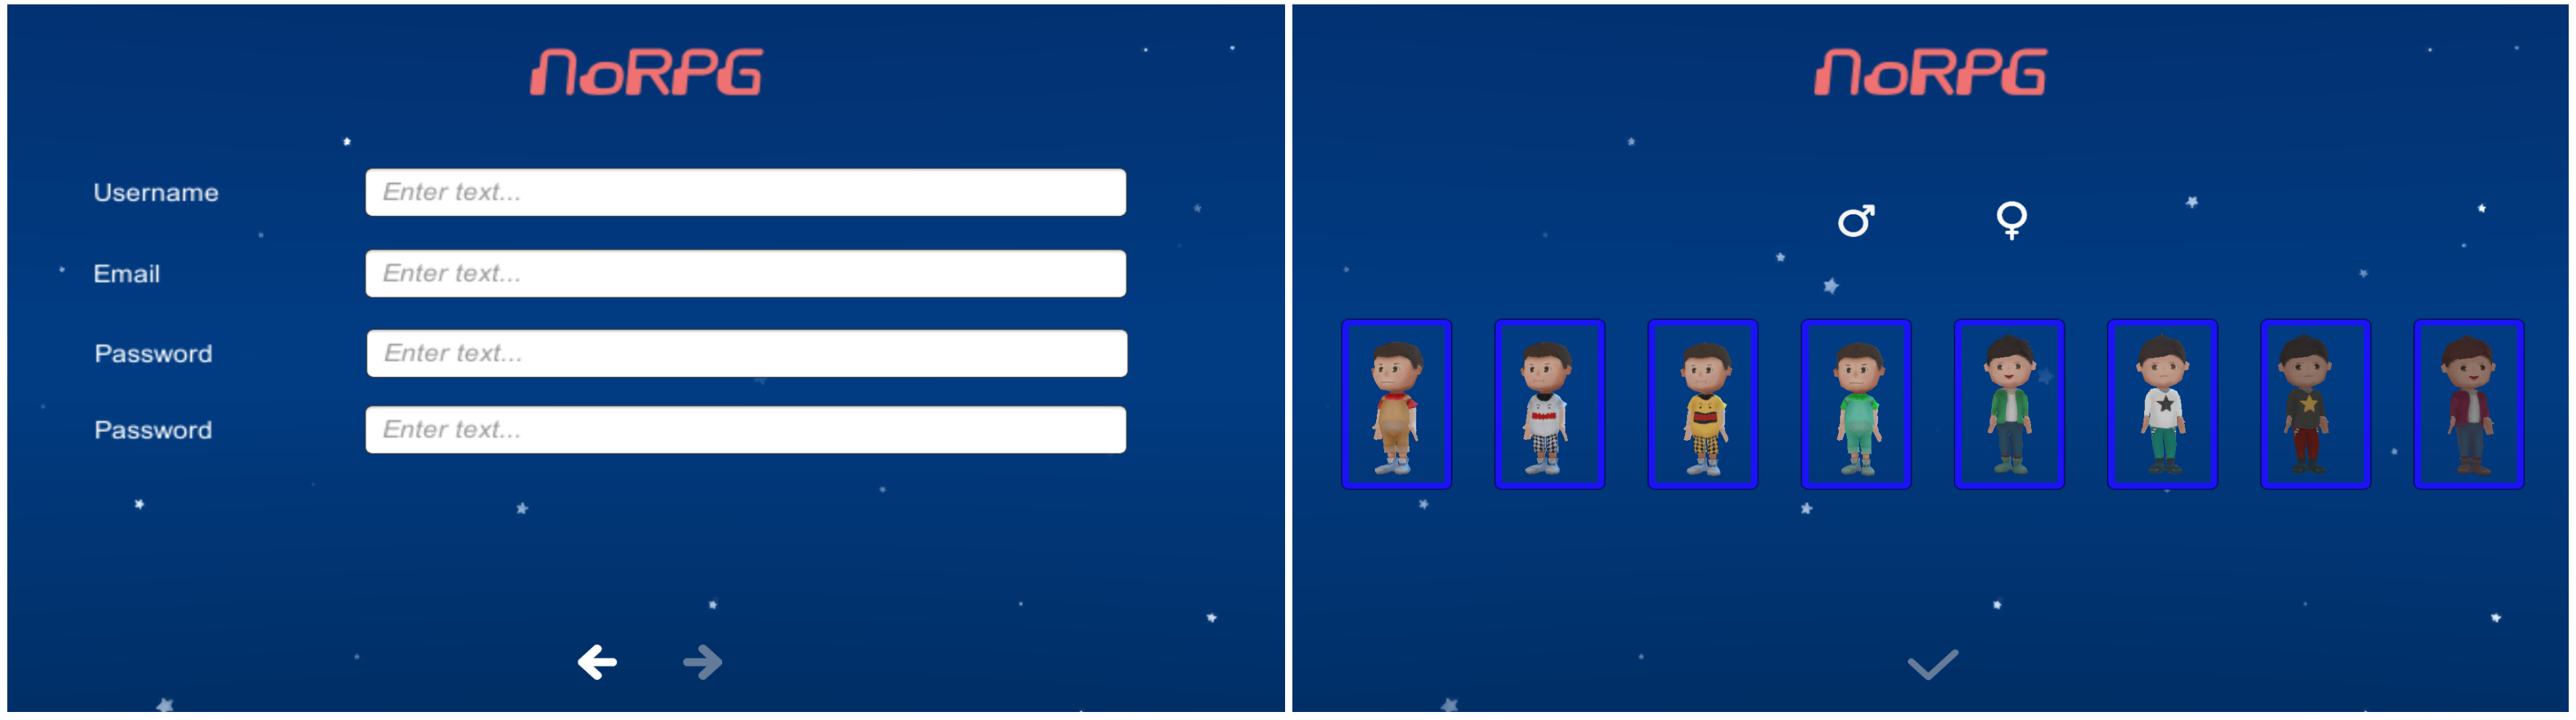
\includegraphics[width=\textwidth]{pics/registerScreen.png}
					\caption{User Interface: Registrierung}
				\end{figure}

				Es fällt auf, dass auch hier das Gestaltungsprinzip Ground/Figure umgesetzt wurde. Dies hat die gleichen Gründe wie bei den Startbildschirmen und die Konsistenz außerhalb des eigentlichen Spieles bleibt erhalten. Neben diesen Gestaltungsprinzip wurde versucht das Prinzip Simple und Clean weiter fortzuführen, allerdings handelt es sich bei der Registrierung um einen komplexeren Prozess. Daher wurde ein weiteres Gestaltungsprinzip verwendet. 
				
				Die \ac{UI} Elemente sind tabellarisch angeordnet und deren relative Abstände gruppieren einzelne Elemente. Dieses Prinzip wird Proximity genannt. Dadurch weiß der Spieler welche Eingabefelder zu welchen Textfeldern gehören und kann somit die korrekten Informationen angeben. Auch hier ist das User Interface in zwei Abschnitte unterteilt. Der erste Abschnitt ist in der Mitte des Bildschirms positioniert und bildet das Registrierungsformular ab. Der zweite Abschnitt ist am unteren Teil des Bildes und dient zur Navigation durch den gesamten Registrierungsprozess.

				Der größte Unterschied ist allerdings, dass diese Szene mit dem Render-Modus World Space implementiert wurde. Der letzte Schritt im Registrierungsprozess ist die Auswahl des Charakters. Damit die einzelnen Charaktere in die \ac{UI} integriert werden konnten, musste dieser Modus umgesetzt werden. Dadurch wurde möglich, dass zunächst die 3D Objekte der Welt nicht von den \ac{UI} Elementen verdeckt werden und anschließend kann der Spieler auf seinen gewünschten Charakter klicken und es wird eine Animation ausgeführt. 

			\subsubsection{\acl{HUD} im Spiel}
				Das \ac{HUD} bildet das User Interface innerhalb des Spieles ab. Grundsätzlich kann das \ac{HUD} in vier Abschnitte unterteilt werden. Die Abschnitte sind an den Ecken des Bildschirmes positioniert. Diese Positionierung hat den Vorteil, dass die \ac{UI} Elemente nicht vom Spiel ablenken und Informationen verdecken, sowie der Spieler die Elemente einfach mit den Händen erreichen kann. Abbildung \ref{alwaysOnUI} stellt die standardmäßige Ansicht von NoRPG dar.

				\begin{figure}[htbp]
					\centering 
					\label{alwaysOnUI}
					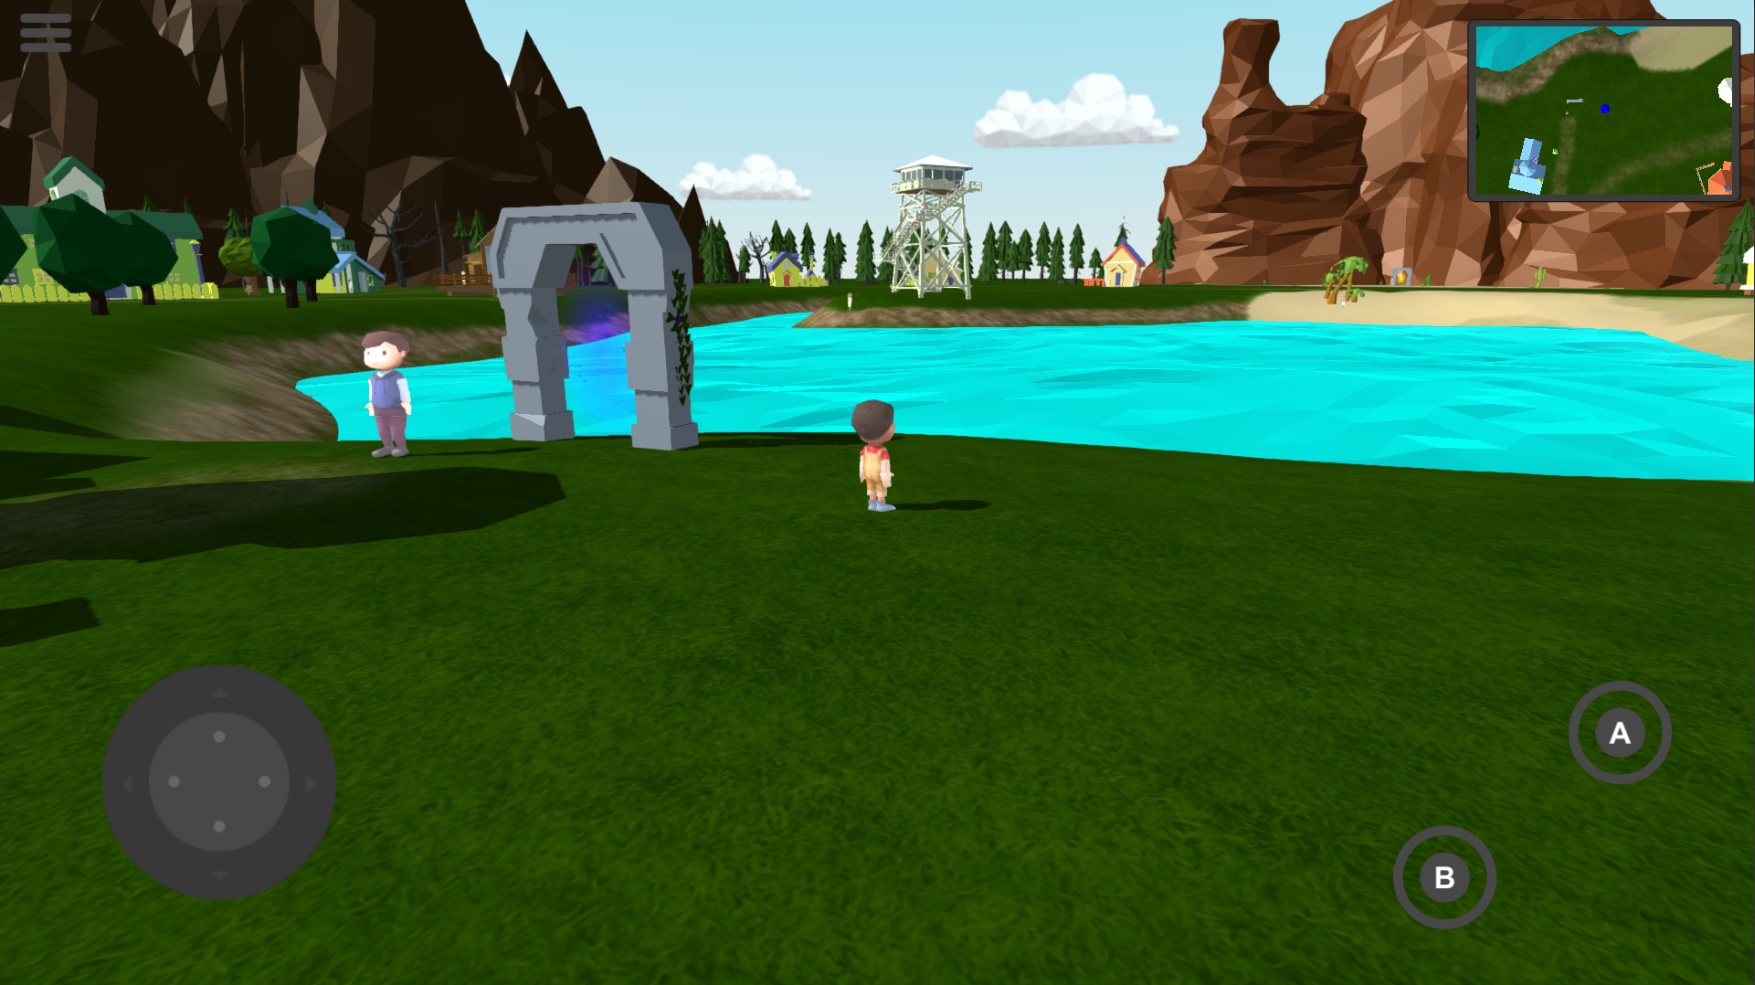
\includegraphics[width=13cm]{pics/alwaysOnUI.png}
					\caption{User Interface: Head-Up Display}
				\end{figure}

				Das ganze \ac{HUD} ist mit dem Render Modus Screen Space - Overlay implementiert. Das \ac{HUD} steht nicht im Fokus, darf allerdings nicht durch 3D Objekte verdeckt werden. Die \ac{HUD} Elemente dienen zur Steuerung des Spieles und sind genauso wichtig wie das Spiel selber.

				\paragraph{Der Joystick}
					Der Joystick befindet sich in der unteren linken Ecke. Der Spieler kann mit Hilfe des Joysticks sich im Spiel fortbewegen. Von allen \ac{UI} Elementen die NoRPG implementiert wurden, ist der Joystick das einzige Elemente, das nicht standardmäßig von Unity zur Verfügung stellt. Bei dem Joystick handelt es sich um ein Asset, welches aus dem Unity Asset Store erworben wurde. Die Besonderheit ist, dass der Joystick aus drei Elementen besteht, welche übereinander liegen. 

					Das oberste Element ist der sogenannte Stick. In der Abbildung \ref{alwaysOnUI} handelt es sich um kreisförmige hellgraue Element in der linken Ecke. Der Spieler interagiert mit dem Stick und kann diesen in alle Richtungen bewegen. Diese Bewegungen werden dann anschließend mit Einsatz eines Skriptes an den Charakter im Spiel übergeben. 

					Bei dem zweiten Element handelt es sich um die Basis des Joysticks. Bei Bewegungseingaben des Spielers ändert sich die Position nicht. Die Basis dient zum einen der Orientierung und begrenzt den Radius des Sticks. Je nachdem wie weit außerhalb der Stick sich innerhalb dieses Radius befindet, bewegt sich der Charakter mit einer unterschiedlichen Geschwindigkeit.

					Das unterste Elemente wird als Touch Zone bezeichnet. Diese ermöglicht innerhalb eines festgelegten Bereiches, dass der Spieler seinen Daumen in eine beliebige Position setzen kann und der Joystick wird genau unter seinem Daumen platziert. Dadurch wird gewährleistet, dass junge Spieler, die eher kleinere Hände haben, und Erwachsene komfortabel den Joystick verwenden können.

				\paragraph{Die Interaktionbuttons}
					Bei den Interaktionsbuttons handelt es sich um die Buttons, die für die Steuerung der Interaktionen in NoRPG zuständig sind. Diese sind an der unteren rechten Ecke positioniert. Es wird zwischen zwei Buttons mit unterschiedlichen Zuständigkeiten unterschiedenen. Der rechte Button, der A-Button, ist für das Starten einer Interaktion und für das Akzeptieren bei Entscheidungsfällen verantwortlich. Der zweite Button, der B-Button, wird zum Abbrechen von Interaktionen benötigt. Allerdings gibt es Situationen, in denen beide Buttons die gleiche Funktionalität abbilden, beispielsweise am Ende einer Konversation kann der Spieler mit beiden Buttons diese beenden. Eine Konversation ist in Abbildung \ref{userInterfaces} im oberen linken Teil abgebildet.

					Damit jedoch nicht immer irgendeine Interaktion gestartet wird, wenn der Spieler die Taste verwendet, wurde ein Skript implementiert, der den Abstand vom Spieler zum nächsten Objekt im Spiel bestimmt. Erst wenn der Spieler sich in der Nähe des Objektes befindet, wird eine Interaktion gestartet. Dies wird später im Kapitel 5.4.4 genauer behandelt.

					Bei den Buttons handelt es sich um standardmäßige Buttons von Unity. Allerdings sind diese mit einer animierbaren Textur überzogen. Die Textur verändert das aussehen des Buttons und ermöglicht visuelles Feedback zurückzugeben, falls der Button geklickt wird oder für einen Moment nicht benutzbar ist.

					\begin{figure}[htbp]
						\centering 
						\label{userInterfaces}
						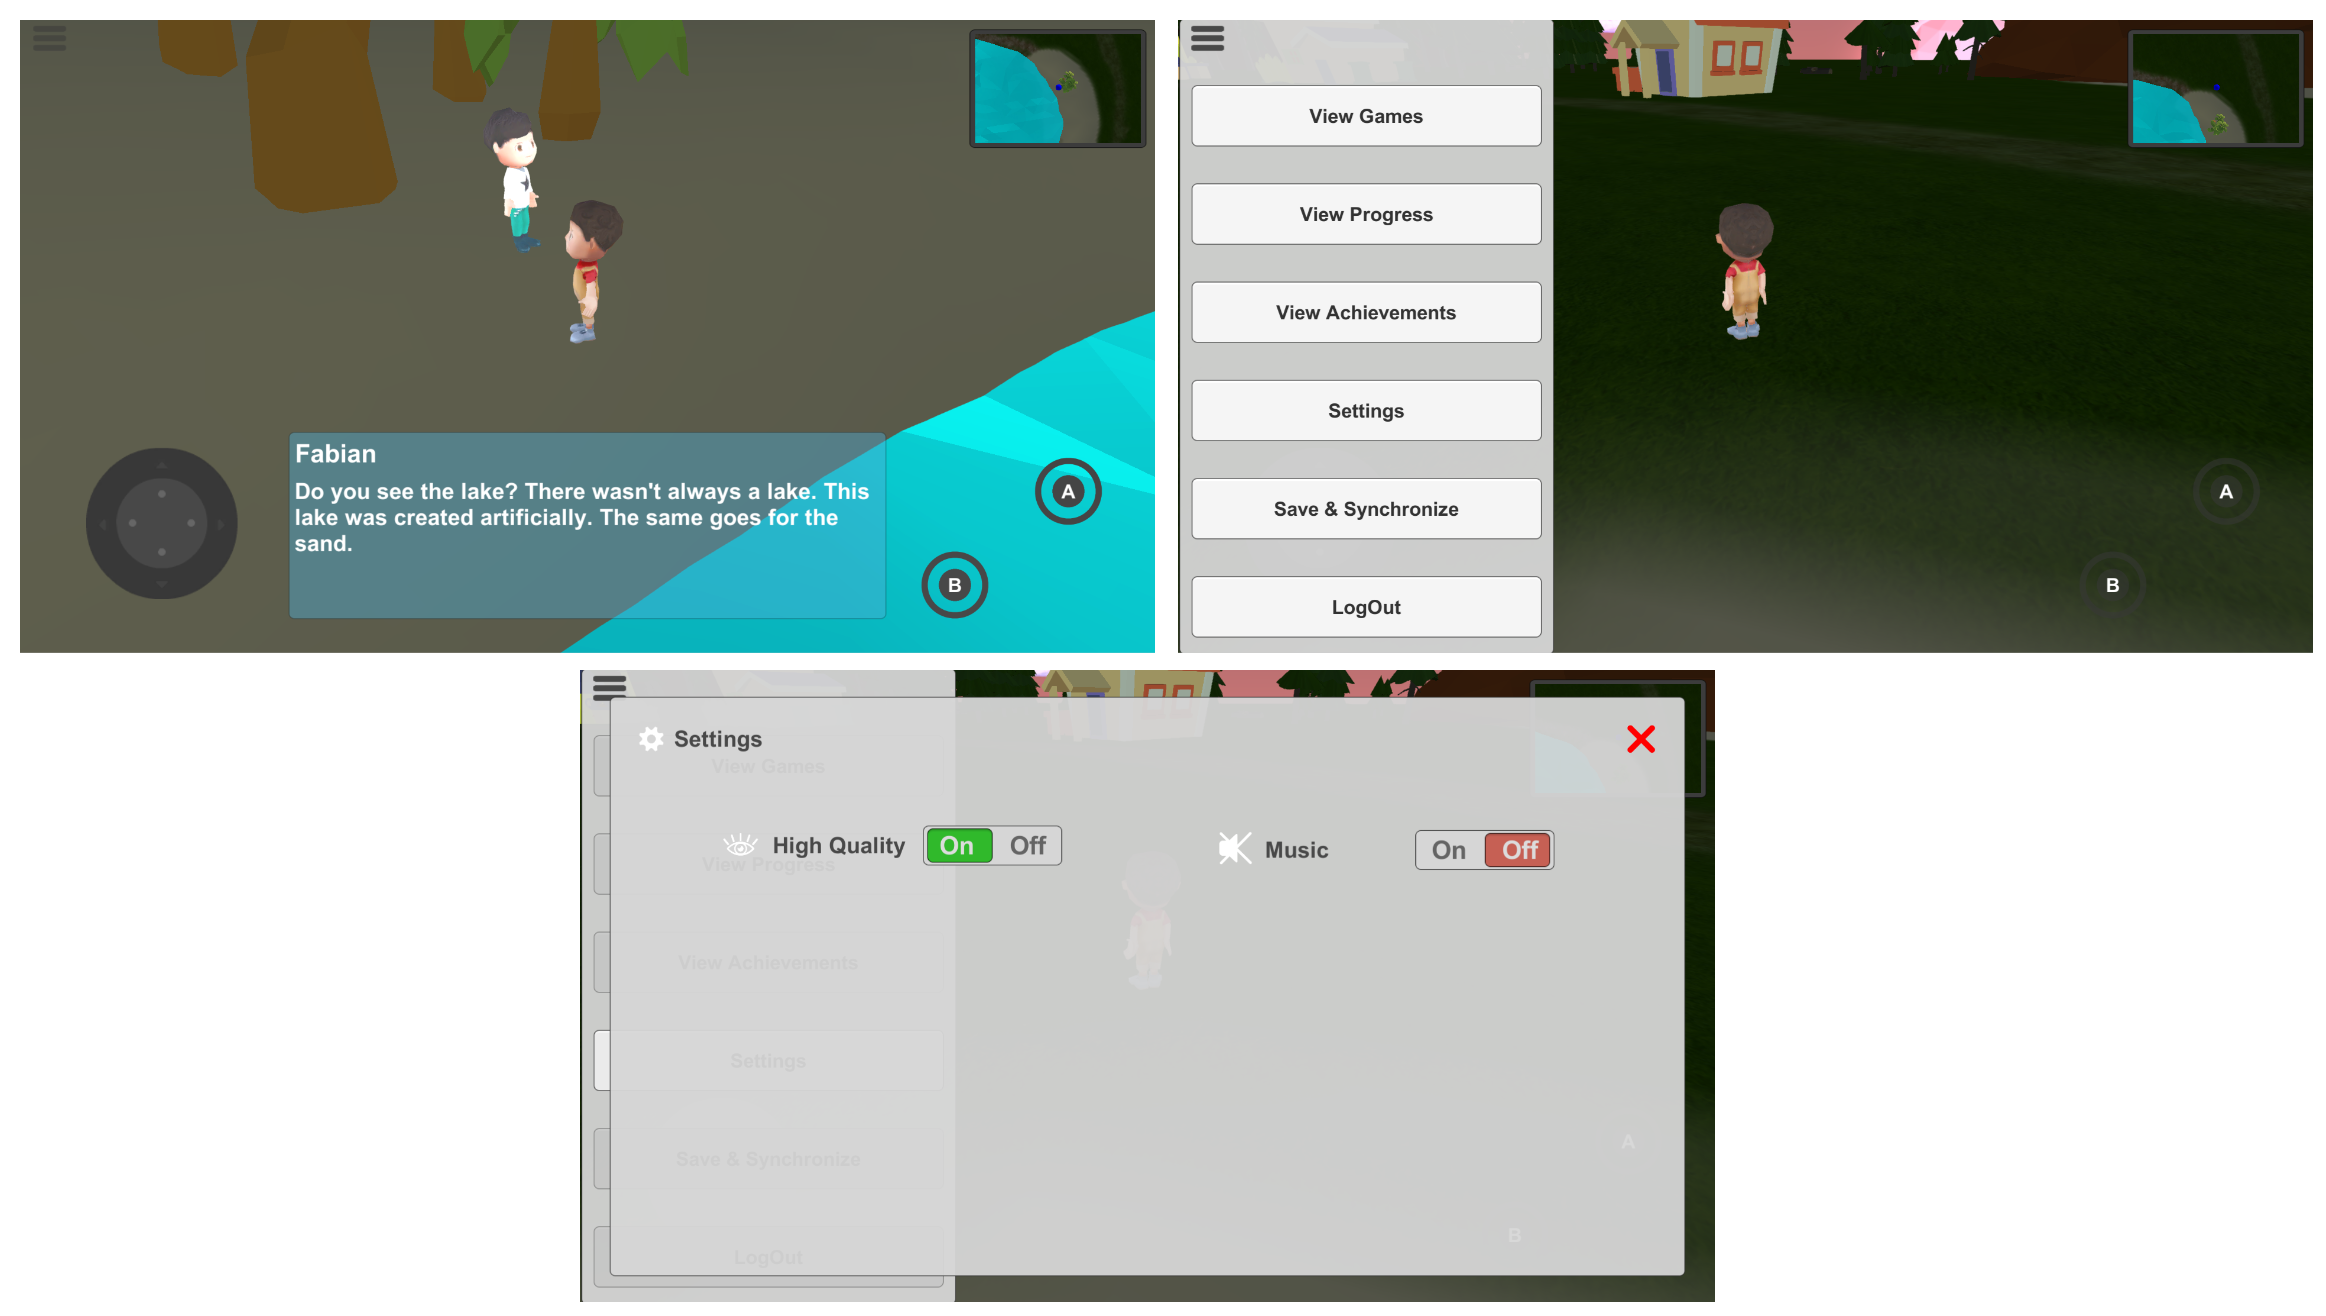
\includegraphics[width=\textwidth]{pics/userInterface.png}
						\caption{User Interfaces: Kommunikation, Menü und Einstellungen-Fenster}
					\end{figure}

				\paragraph{Das Menü}
					Der Button für das Menü befindet sich in der oberen linken Ecke. Dieser ist im oberen Teil des Bildschirms positioniert, da die Häufigkeit der Benutzung wesentlich geringer ist, als bei den bisher besprochenen \ac{UI} Elementen.

					Bei der Verwendung des Buttons öffnet sich das Menü im linken Teil des Bildschirms. Dies im unteren linken Bild der Abbildung \ref{userInterfaces} abgebildet. Das geöffnete Fenster beinhaltet alle restlichen Funktionen, die nicht direkt über das \ac{HUD} erreicht werden können. Beispielsweise findet der Spieler die Einstellungen oder kann seinen Fortschritt öffnen. Diese Funktionen sind in dem Menü, da die Informationen nicht immer benötigt werden und deshalb nicht die ganze Zeit sichtbar sein müssen. Während das Menü offen ist können keine anderen \ac{UI} Elemente, wie die Buttons zur Interaktion verwendet werden. Der Spieler muss erst das Menü schließen um wieder mit dem Spiel fortfahren zu können. 

					Es wird zwischen zwei Varianten von Funktionen im Menü unterschieden. Einige der Funktionen öffnen ein weiteres Fenster, wie in der Abbildung \ref{userInterfaces} im unteren rechten Bild abgebildet, und andere werden direkt im Menü ausgeführt. So wird beispielsweise für die Einstellungen ein weiteres Fenster geöffnet, wohingegen das Speichern direkt im Menü durchgeführt wird, ohne das sich ein Fenster öffnet.

				\paragraph{Die Karte}
					Die Karte im oberen rechten Eck des Bildschirms wird als Mini Map bezeichnet. Sie bietet dem Spieler einen Überblick über seine aktuelle Position. Realisiert wurde diese Mini Map mit einer zusätzlichen zweiten Kamera, die von oben auf den Spieler schaut. Das Objekt der Mini Map ist am Charakter angebracht, damit der Spieler und die Mini Map sich immer in der gleichen Position befinden.

					Da zwei Kameras die Komplexität der Szene erhöhen, indem alle Bilder doppelt dargestellt werden, muss die zusätzliche Kamera angepasst werden. Diese rendert die Szene nicht mit der gleichen Qualität wie die Hauptkamera. Des Weiteren werden einige Elemente, wie beispielsweise Schatten oder zu kleine 3D-Objekte wie Blumen nicht in der Mini Map gerendert. 

					Der Spieler kann auf die Mini Map klicken und es wird die komplette Karte der aktuellen Spielwelt geöffnet. Diese Übersicht wird ebenfalls mit einer Kamera aufgenommen. Der Unterschied allerdings ist, dass diese Kamera nur eingeschaltet ist, also nur dann rendert wenn der Spieler auf die Mini Map klickt. Die Karte kann in Abbildung \ref{userInterfaces} im oberen rechten Bild betrachtet werden.

					Die Kamera ist nicht wie die Mini Map am Spieler angebracht, sondern schwebt über der ganzen Szene. Die Karte zeigt ebenfalls keine Schatten oder zu kleine Objekte an, wodurch Ressourcen gespart werden.

					Während die Karte offen ist kann der Spieler nicht das Menü öffnen oder eine Interaktion starten, allerdings kann sich der Spieler mit dem Joystick bewegen. Die Kamera dient zur Orientierung in der Spielwelt, deshalb darf der Spieler sich bewegen. Die Karte kann während dem Laufen geöffnet und geschlossen werden.

		\subsection{Usability Evaluation}
			Ein Usability Test wird durchgeführt, um die Gebrauchstauglichkeit einer Software oder Hardware mit den potenziellen Benutzern zu überprüfen. Usability wird durch die Attribute Erlernbarkeit, Effizienz, Einprägsamkeit, Fehlerrate und Zufriedenheit\footnote{Vgl. Nielsen \cite{NielsenUI} Seite 26} beschrieben. Unter dem Attribut Erlernbarkeit beschreibt Nielsen in seinem Buch, dass die Anwendung leicht zu erlernen sein muss, damit der Benutzer in kurzer Zeit beginnen kann das Spiel zu spielen. Dazu zählt beispielsweise die Steuerung. Diese ist wichtig, damit der Benutzer sich im Spiel intuitiv bewegen kann. So bald der Spieler das System gelernt und verstanden hat, soll ein hohes Maß an Produktivität möglich sein. Dies wird als Effizienz bezeichnet. Das System sollte allerdings leicht zu merken und einprägsam sein, so dass auch der Gelegenheitsbenutzer in der Lage ist, nach einer gewissen Zeit ohne Verwendung der Anwendung, in das Spiel zurückzukehren, ohne alles nochmals neu lernen zu müssen. Nielsen weißt zudem darauf hin, dass Fehler für den Benutzer sehr frustrierend sein können. Daher sollte das System eine geringe Fehlerquote haben, so dass Benutzer bei der Verwendung nur wenig Fehler machen und falls Probleme auftauchen, diese den Spaß am Spielen nicht einschränken\footnote{Vgl. Nielsen \cite{NielsenUI} Seite 27ff.}. Das letzte Attribut beschreibt den Gesamteindruck.

			Es wird zwischen formativem und summativem Usability Test unterschieden. Foramtive Tests werden während der Entwicklung durchgeführt. Die Aufgabe ist es ein spezielles Problem bzw. Szenario zu testen. Es handelt sich dabei um eine kleine Studie für schnelles Feedback, welche wiederholt durchgeführt werden kann\footnote{Vgl. Rubin und Chisnell \cite{handbookUsability} Seite 29f.}. Der summative Test findet einmalig nach der Entwicklung statt, bevor das fertige Produkt ausgeliefert wird. Dabei handelt es sich um eine umfangreiche Studie, die alle Funktionen der Benutzeroberfläche bewertet\footnote{Vgl. Rubin und Chisnell \cite{handbookUsability} Seite 34f.}.

			Ein Usabilty Test kann in verschiedenen Testumgebungen durchgeführt werden. Es wird zwischen Labortest, Feldtest und Remotetest unterschieden. Bei einem Labortest handelt es sich entweder um ein Usability Labor oder um einen allgemein nutzbaren Raum. Der ausschlaggebende Unterschied zwischen diesen beiden ist, dass das Usability Labor nur für Usabilty Tests und Evaluationen verwendet wird. Die potenziellen Tester werden eingeladen und führen die Auswertung in diesem Raum durch. Zu den Basisutensilien gehört neben Nahrung und Verpflegung die notwendige Hardware und Software, sowie ein Moderator bzw. Experte für Fragen und Probleme\footnote{Vgl. Rubin und Chisnell \cite{handbookUsability} Seite 101f.}. Der Feldtest oder auch Mobiler Test kann potentiell überall durchgeführt werden, sei es beim Kunden, in einem öffentlichen Gebäude oder in einem Café. Der Vorteil im Vergleich zu einem Labortest ist, dass der Benutzer sich einer gewohnten und reale Umgebung mit echten Lichtverhältnissen befindet. Allerdings ist es wahrscheinlicher das der Tester durch die Umwelt abgelenkt wird\footnote{Vgl. Rubin und Chisnell \cite{handbookUsability} Seite 98f.} und der Experte mit zum Kunden. Bei der letzten Möglichkeit ist der Benutzer und Moderator örtlich voneinander getrennt. Der Remotetest kann synchron, indem der Moderator und die Teilnehmer per Audio- oder Videokonferenz verbunden sind, oder asynchron stattfinden. Der wesentliche Vorteil ist, dass dadurch potenziell mehr Testpersonen teilnehmen und es günstiger ist. Allerdings können keine komplexen Anforderungen gestellt werden und bei Fragen ist der Tester mehr oder weniger auf sich gestellt.

			\subsubsection{Vorbereitung und Durchführung}
				Bei der in diesem Kapitel beschrieben Evaluation handelt es sich um einen summativen Remotetest. Der Usability Test findet erst nach der Entwicklung von NoRPG statt und nachdem alle Funktionen implementiert wurden. Die Gründe für einen Remotetest sind, da eine es sich bei NoRPG um eine mobile Anwendung handelt und diese am besten auf dem eigenen Smartphone getestet werden kann. Dadurch werden auch verschiedenste Hardware und Android Versionen geprüft und validiert. Ein weiterer essentieller Punkt sind die Kosten. In dem Umfang dieser Studienarbeit ist es nicht möglich ein Feldtest oder Labortest durchzuführen.

				In der Vorbereitung des Usability Tests gilt es zunächst die Benutzerprofile zu erstellen, die zu testenden Szenarien und Ziele, sowie den Umfang zu definieren. Anschließend die Unterlagen vorzubereiten, die Teilnehmer zu rekrutieren und den Zeitraum festzulegen. Das Profil für die Tester ist das gleiche wie das der potenziellen Spieler. Daher wird kein festes Profil für die Evaluation festgelegt, da NoRPG für jung oder alt und männlich oder weiblich ausgelegt ist. Jedoch gilt bei der Rekrutierung zu beachten, das von jeder Alters- und Geschlechtsgruppe eine gewisse Anzahl vertreten ist.

				Das Ziel dieser Evaluation ist das Testen der Benutzeroberfläche, da es sich bei einer mobilen Anwendung um die einzige Interaktionsschnittstelle für die Benutzer handelt. Aus diesem Grund ist eine fehlerfreie, intuitive und gleichzeitig gut aussehende Benutzeroberfläche sehr wichtig. Zu den abzubildenden Szenarios gehört zum Beispiel die Registrierung, der Log-In oder die Liste der heruntergeladenen Spiele. Alle \ac{UI} Elemente sollen in diesem summativen Test geprüft und evaluiert werden und aus diesem Grund ist der Umfang dieser Evaluation größer. Diese findet in dem Zeitraum 24.04.2017 bis 30.04.2017 statt.

				Für die Evaluation wurde ein Dokument für die Tester erstellt. Dieses beinhaltet alle notwendigen Information und ist zugleich eine Schrittanleitung, um alle \ac{UI} Elemente testen zu können. Ein ausgefülltes Formular\ref{ueMarcel}, dessen Publikation von dem Tester genehmigt wurde, befindet sich im Anhang dieser Arbeit. Neben den Informationen gibt es mehrere Spalten, die für die Bewertung dienen. Bewertet werden kann ein Szenario mit "++", "+", "0", "\-" und "\--".

			\subsubsection{Bewertung}
				Für die Evaluation von NoRPG wurde an alle potenzielle Tester eine Prerelease Version der App und der auszufüllende Bewertungsbogen verteilt. Weitere Anweisungen wurden nicht mitgeteilt.

				Zunächst werden alle zusätzlichen Informationen, die aus den Fragebögen gewonnen werden konnten, behandelt und deren Verteilung betrachtet.

				Bei dem durchschnittlichen Tester handelt es sich um einen 19 Jahre alten männlichen Tester aus Deutschland. Diese Aussage beruht auf der Auswertung des Fragebogens, welche in Abbildung \ref{auswertungTester} abgebildet sind. Von allen teilnehmenden Testern sind davon 81\% männlich und die übrigen 19\% weiblich. Für die Auswertung wurden drei Altersgruppen definiert und festgelegt. Die meisten Teilnehmern waren über 20 Jahre, da die Evaluation von Kindern alleine schwer ausgefüllt werden kann. Die jüngeren Tester haben mit Hilfe einer Aufsichtsperson NoRPG getestet und das Ergebnis in der Evaluation festgehalten. Der Großteil der Tester kommt aus Deutschland, allerdings ergab sich die Möglichkeit, einige Tester aus der Türkei zu gewinnen. Diese Erkenntnisse haben Einfluss und Bedeutung in der Bewertung von NoRPG.

				\begin{figure}[htbp]
					\centering 
					\label{auswertungTester}
					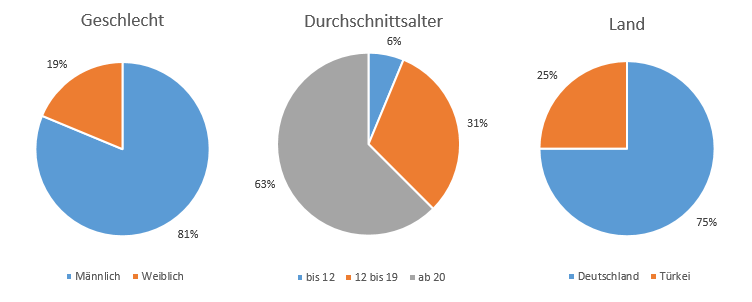
\includegraphics[width=\textwidth]{pics/TesterAuswertung.png}
					\caption{Evaluation Auswertung - Der durchschnittliche Teste}
				\end{figure}

				Neben dem Alter, Geschlecht und Herkunftsland konnten die Tester zudem auch die Marke des Smartphone-Herstellers und die installierte Android Version angeben. Dies hat den Zweck, ob die Einschränkungen im \ac{SRS} im Vorhinein korrekt und sinnvoll waren. Das Ergebnis ist in der Abbildung \ref{auswertungSmartphones} zu sehen. Mit einem Anteil von 50\% ist die am häufigste verbreitete Smartphone Marke die des Herstellers Samsung. Auf den Smartphones war im Durchschnitt am meisten Android 7 installiert. Allerdings gibt es ein Unterschied zwischen den installierten Android Versionen. Die Testen in Deutschland hatten überwiegend die Version 7.x installiert, wohingegen in der Türkei diese Version auf keinem Testgerät installiert war.

				\begin{figure}[htbp]
					\centering 
					\label{auswertungSmartphones}
					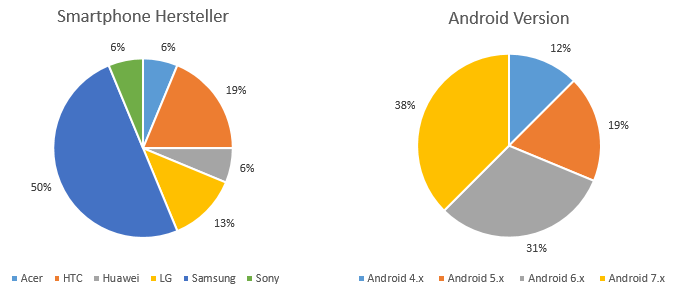
\includegraphics[width=\textwidth]{pics/SmartphoneAuswertung.png}
					\caption{Evaluation Auswertung - Die durchschnittliche Hard- und Software}
				\end{figure}

				Im folgenden Abschnitt dieses Kapitels wird nun das Ergebnis der Evaluation behandelt und ausgewertet. Der einzelnen Szenarien konnten von den Testern von "\-- -"\ bis "++" bewertet werden, während "++" die beste Bewertung darstellt. Damit das Ergebnis die Bewertung von allen Testern widerspiegelt, wurde "\-- -"\ mit -2 und "++" mit +2 verrechnet. Dies kann in Tabelle \ref{tab:ergbnisOverall} betrachtet werden. Diese entspricht dem des Bewertungsbogens, allerdings ohne nähere Beschreibung der einzelnen Szenarien. Die Punktzahl in der letzten Spalte spiegelt den genauen Durchschnitt von allen Testern wider.

\begin{table}[htbp]
	\centering
	\begin{tabular}{|l|l|c|c|c|c|c|c|}
		\hline
		\multirow{2}{*}{Szene} & \multirow{2}{*}{Szenario} &\multicolumn{5}{c}{Bewertung} \vline & \multirow{2}{*}{Punkte} \\ 
		& & -- & - & 0 & + & ++ & \\ \hline
		\multirow{3}{*}{Startscreen (Logged Out User)} & Log-In &  &  &  & x &  & 1,4 \\ 
		& Change Settings &  &  &  & x &  & 1,32 \\ 
		& Register &  &  &\multicolumn{2}{c}{x} \vline &  & 0,7 \\ \hline 
		\multirow{2}{*}{Registerszene} & Create new Account &  &  &  & x &  & 1,1 \\ 
		& Cancel Registration &  &  &  & x &  & 1 \\ \hline 
		\multirow{3}{*}{Startscreen (Logged In User)} & Log-In &  &  &  &\multicolumn{2}{c}{x} \vline & 1,6 \\ 
		& Log-Out &  &  &  & x &  & 1 \\ 
		& Change Settings &  &  &  & x &  & 1,3 \\ \hline 
		\multirow{10}{*}{Head Up Display} & Overview &  &  &  &\multicolumn{2}{c}{x} \vline & 1,6 \\  
		& Move Character &  &  &  & x &  & 1,4 \\  
		& Start Interaction &  &  &  & x &  & 1,3 \\  
		& Open Map &  &  &  &  & x & 1,7 \\  
		& Open Menu &  &  &  & x &  & 1,3 \\  
		& View Games &  &  &  &\multicolumn{2}{c}{x} \vline & 0,6 \\  
		& View Progress &  &  & x &  &  & 0,4 \\
		& View Achievements &  &  &  & x &  & 0,9 \\ 
		& Change Settings &  &  &  & x &  & 0,8 \\ 
		& Log-Out &  &  &  & x &  & 1 \\ 
		\hline
	\end{tabular}
	\caption{Ergebnis der Evaluation - Die Bewertung}
	\label{tab:ergbnisOverall}
\end{table}

				Zunächst kann behauptet werden, dass die Auswertung positiv ausgefallen ist. Wenn alle Punkte von den einzelnen Szenarien zusammen betrachtet werden, ergibt es das Ergebnis von 1,1, welches in der Bewertungsmatrix unter "+" fallen würde.

				Sehr positiv aufgenommen haben die Tester das Aussehen der \ac{UI} Elemente. Durch die Darstellung der Funktionen mit bekannten, allerdings auch modernen, Symbolen konnten die auszuführende Aktion mit dem Element assoziiert werden. Ebenfalls damit verbunden wird das konsistente Aussehen sehr positiv beschrieben. Obwohl so viele Funktionen im Spiel möglich sind, ist die Komplexität des Spieles sehr gering. Dies sticht in der Bewertung insbesondere mit dem Szenario "Open Map" hervor. Durch einen einfachen Klick auf die Karte vergrößert sich die Karte und der Spieler kann die ganze Spielwelt betrachten.

				Allerdings gibt es je nach Benutzergruppe Auffälligkeiten und Unterschiede in den Bewertungen. So haben eher jüngere Teilnehmer meistens nur auf das Aussehen der \ac{UI} Elemente geachtet und benötigten bei der Registrierung die Unterstützung eines Erwachsenen. Die schlechteste Bewertung erhielt das Szenario "View Progress". Diese beschreibt, dass der Spieler seinen Fortschritt und seine gelernten Standards betrachten will. Jedoch war diese Information für die jüngeren irrelevant und eher verwirrend.

				Im Gegensatz dazu haben die älteren Tester zudem neben dem Aussehen auch beispielsweise die Eignung und eher kritischer bewertet. Es wurde häufig angemerkt, das wichtige Informationen farblich hervorgehoben werden sollten und das zum Beispiel vor der Abmeldung der Spieler darauf hingewiesen werden.

				Große Unterschiede zwischen den Bewertungen von männlichen und weiblichen Testern gab es keine. Jedoch konnten Unterschiede zwischen den Ländern festgestellt werden. So wurde das User Interface eher besser von deutschen Testern verstanden.

				Viele dieser Anmerkungen, wie beispielsweise ein Dialog bei der Abmeldung oder andere eher kleinere Vorschläge wurden nach der Evaluation implementiert.

	\section{C\# Skripte}
		Nachfolgend wird auf einzelne C\# Skripte eingegangen, welche essentiell für die korrekte Ausführung der App benötigt werden. Neben den Skripten wird auch auf weitere Komponenten für die Skripte eingegangen.

		\subsection{Player}
			Der Player ist das Objekt, welches vom Spieler bewegt wird und ist für die Interaktion mit der kompletten Umgebung zuständig. Das Objekt setzt sich aus mehreren einzelnen Unterkomponenten zusammen, darunter fällt zum einen die Textur des Charakters, ein Teil der Minimap und ein Objekt für die Kamera. 
	
			An dem Elternobjekt Player sind Skripte und von Unity zur Verfügung gestellt Objekte angebracht. Zu diesen Objekten gehören der Rigidbody, CharacterController, Animator und ThridPersonController. Der Rigidbody sorgt dafür, dass der Player Gravitation erfährt und nicht einfach durch die Luft schweben kann. Der CharacterController implementiert verschiedene Eigenschaften, wie beispielsweise die Breite, Höhe und den Schrittversatz. Der Schrittversatz bestimmt über welche Höhen und Objekte, wie beispielsweise Treppenstufen, der Player laufen kann. Der Animator ist zusammen mit dem ThirdPersonController dafür verantwortlich, dass sich der Player in der Szene bewegt und die Bewegungsanimationen korrekt ausgeführt werden. 
	
			Daraus resultieren folgende Möglichkeiten der Animation:

 \begin{table}[htbp]
 \centering
 \begin{tabular}{|c|c|l|}
 \hline
  speed & direction & Ergebnis \\
 \hline
  0 & 0 & Animation Idle \\
  >0 & 0 & Animation Walk \\
  >0 & 0.3 & Animation Walk Right Short \\
  >0 & 0.5 & Animation Walk Right Medium \\
  >0 & -0.3 & Animation Walk Left Short \\
  >0 & -0.5 & Animation Walk Left Medium \\
  >0.5 & 0 & Animation Run \\
  >0.5 & 0.3 & Animation Run Right Medium \\
  >0.5 & 0.5 & Animation Run Right Wide \\
  >0.5 & -0.3 & Animation Run Left Medium \\
  >0.5 & -0.5 & Animation Run Left Wide \\ \hline
 \end{tabular}
  \caption{Mögliche Animationen je nach Wert speed und direction}
 \label{tab:tabspeeddirection}
 \end{table}
 
			Erst durch diese Vielzahl an Animationen wird gewährleistet, dass der Player zu jeder Zeit die richtige Animation ausführt und die Bewegungen nicht unnatürlich aussehen. Damit dies passiert, werden die Werte speed und direction vom in Kapitel 5.3.1 besprochenen Joystick im Skript CharacterControll.cs an den Charakter übergeben. Diese ist für die Steuerung des Players zuständig. Hier wird die Toucheingabe über den Joystick in Weltkoordinaten umgewandelt und der Player beginnt sich zu bewegen. Das Skript ist in Listing \ref{lst:charactercontroller} aufgeführt.
	
			Dazu wird die Methode Update genutzt. In dieser wird, sofern ein Animator an dem Player vorhanden ist, die horizontale und vertikale Bewegung des Joysticks in die Werte für direction und speed umgewandelt. Das ganze passiert dabei in der Methode StickToWorldspace in Zeile 32. 

			In der Methode wird zu Beginn die rootDirection gesetzt, welche sich dabei aus der Z-Achsen Koordinate zusammensetzt. Anschließend wird die stickDirection durch den horizontalen und vertikalen Wert des Joysticks gesetzt. Abschließend wird der Wert von speed durch die Quadrierung der beiden Werte berechnet. Dieser liegt dabei zwischen Null und Eins. Danach wird das ganze in Bezug zu der Positionsrichtung der Kamera gesetzt, um die Bewegungsrichtung zu erhalten und anschließend das Kreuzprodukt aus diesen beiden Werten zu berechnen. Mit Hilfe des Wertes kann bestimmt werden, ob sich der Player nach Rechts oder nach Links bewegen soll.
	
			Nachdem diese aufgerufen wurde und abgeschlossen ist, werden die Werte von direction und speed an den ThridPersonController übergeben und die korrekte Animation wird startet.

\begin{scriptsize}
\lstset{
	float,
	caption=CharacterController.cs, 
	language=[Sharp]C, 
	frame=single,  
	showstringspaces=false, 
	showspaces=false, 
	numbers=left, 
	captionpos=b, 
	belowcaptionskip=4pt,
	basicstyle=\ttfamily
} 
\begin{lstlisting}[label=lst:charactercontroller]
public class CharacterControll : MonoBehaviour {
  [...]	
	
  void Update() {  
    if (animator) {
      stateInfo = animator.GetCurrentAnimatorStateInfo(0);
      horizontal = CnInputManager.GetAxis("Horizontal");
      vertical = CnInputManager.GetAxis("Vertical");
      
      StickToWorldspace(this.transform, gamecam.transform, ref direction, ref speed);
      animator.SetFloat("speed", speed);
      animator.SetFloat("direction", direction, directionDumpTime, Time.deltaTime);
    }
  }
    
  [...]

  public void StickToWorldspace(Transform root, Transform camera, 
    ref float directionOut, ref float speedOut) {
    
    Vector3 rootDirection = root.forward;
    Vector3 stickDirection = new Vector3(horizontal, 0, vertical);
    speedOut = stickDirection.sqrMagnitude;
    Vector3 CameraDirection = camera.forward;
    CameraDirection.y = 0.0f;
    
    Quaternion referentialShift = Quaternion.FromToRotation(Vector3.forward, 
      Vector3.Normalize(CameraDirection));
        	
    Vector3 moveDirection = referentialShift * stickDirection;
    Vector3 axisSign = Vector3.Cross(moveDirection, rootDirection);
    float angleRootToMove = Vector3.Angle(rootDirection, moveDirection) 
      * axisSign.y >= 0 ? -1f : 1f);      
        	
    angleRootToMove /= 180f;
    directionOut = angleRootToMove * directionSpeed;
  }
}
\end{lstlisting}
\end{scriptsize}

		\subsection{Kamera}
			Bei der Kamera handelt es sich um ein Objekt, welches dem Charakter folgt. Dafür ist an dem Player ein Objekt mit dem Namen „follow” angehängt, auf das die Kamera zeigt. 
	
			Die Kamera referenziert das Skript ThirdPersonCamera.cs. In diesem wird das Verhalten der Kamera gesteuert. Dazu werden die Methoden aus dem Listing \ref{lst:lateupdate} verwendet. In LateUpdate in Zeile 4 wird dabei die Position der Kamera in Bezug zum Spieler gesetzt. Dabei befindet sich die Kamera immer in einem Kreis um dem Spieler herum, wodurch die Sicht nicht eingeschränkt wird.

\begin{scriptsize}
\lstset{
	float,
	caption=Methode LateUpdate aus ThirdPersonCamera.cs, 
	language=[Sharp]C, 
	frame=single,  
	showstringspaces=false, 
	showspaces=false, 
	numbers=left, 
	captionpos=b, 
	belowcaptionskip=4pt,
	basicstyle=\ttfamily
} 
\begin{lstlisting}[label=lst:lateupdate]
public class ThirdPersonCamera : MonoBehaviour {
  [...]
  
  void LateUpdate() {
    Vector3 characterOffset = follow.position +  new Vector3(0f, distanceUp, 0f);
    lookDir = characterOffset - this.transform.position;
    lookDir.y = 0;
    
    lookDir.Normalize();
    targetPosition = characterOffset + follow.up * distanceUp - lookDir * distanceAway;
    CompensateForWalls(characterOffset, ref targetPosition);
    smoothPosition(this.transform.position, targetPosition);
    transform.LookAt(follow);
  }

  [...]
  
  private void CompensateForWalls(Vector3 fromObject, ref Vector3 toTarget) {
    RaycastHit wallHit = new RaycastHit();
    if(Physics.Linecast(fromObject, toTarget, out wallHit)) {
      toTarget = new Vector3(wallHit.point.x, toTarget.y, wallHit.point.z);
    }
  }
}
\end{lstlisting}
\end{scriptsize}

			Darüber hinaus wird in LateUpdate unterbunden, dass die Kamera in Wänden verschwindet und durch Objekte geschaut werden kann. Dazu wird die Methode CompensateForWalls in Zeile 21 ausgeführt. In dieser wird getestet, ob zwischen der Kamera und dem Spieler ein Objekt vorhanden ist. Wenn das der Fall ist, wird die Kamera vor dieses Objekt gesetzt.

			Beim aller ersten Start des Spieles gibt es eine geskriptete Szene, in der der Spieler kurz in die Geschichte von NoRPG geführt wird. Dabei wird die Farbe der Startwelt entfernt (siehe Kapitel \ref{geschichte}). Dazu wird ein Shader genutzt, welcher die Farbintensität von jedem Pixel verändert. Das Attribut Intensität des Shaders bestimmt über die Stärke der Graustufen. Dieser wird zu Beginn auf eins gesetzt und für jeden gefundenen Diamanten in den anderen Welten minimiert.
    
		\subsection{Portale}
			Die Portale verbinden die einzelnen Szenen, in denen die verschiedenen Welten abgebildet sind. Diese sind separiert jeweils in einer Szene implementiert, da eine riesige Szene sehr viel Performance benötigen würde.
	
			In der Startwelt sind fünf verschiedene Portale platziert, mit denen der Spieler in die Welten kommt. Dadurch wird uns ermöglicht die einzelnen Klassen voneinander zu separieren. Jede dieser Welten hat ein Portal, welches den Spieler zurück zur Startwelt bringt. Jedes 3D Objekt in der Szene, dargestellt durch ein Steinbogen mit Partikeln, implementiert das Skript \ref{lst:portal}. Dieses Listing sind enthält nur die zwei wichtigsten Methoden für die Portale.

\begin{scriptsize}
	\lstset{
		float,
		caption=PortalToTargetScene, 
		language=[Sharp]C, 
		frame=single,  
		showstringspaces=false, 
		showspaces=false, 
		numbers=left, 
		captionpos=b, 
		belowcaptionskip=4pt,
		basicstyle=\ttfamily
	} 
	\begin{lstlisting}[label=lst:portal]
public class PortalToTargetScene : MonoBehaviour{
  [...]
	
  void OnTriggerEnter(){
    string currentScene = SceneManager.GetActiveScene().name;
    PortalControl.control.cameFrom = currentScene;
    PortalControl.control.currentScene = targetSceneName;
	
    loadingScreen.gameObject.SetActive(true);

    StartCoroutine(LoadLevelWithRealProgress());
  }
	
  [...]

  IEnumerator LoadLevelWithRealProgress(){
    yield return new WaitForSeconds(1);
	
    ao = SceneManager.LoadSceneAsync("Scenes/" + targetSceneName, LoadSceneMode.Single);
    ao.allowSceneActivation = false;

    while (!ao.isDone){
      progBar.value = ao.progress;
	
      if (ao.progress == 0.9f){
        progBar.value = 1f;
        ao.allowSceneActivation = true;
      }
	
      yield return null;
    }
  }
}
	\end{lstlisting}
\end{scriptsize}

			Die erste Methode OnTriggerEnter() wird ausgeführt, sobald der Spieler mit seinem Charakter durch das Portal geht. Dabei kollidiert der Hüllkörper des Charakters mit dem Hüllkörper des Portals und lösen die Funktion aus. Der Hüllkörper in Unity ist als Collider bezeichnet, und umschließt komplexe (nicht Polygone) Objekte, um die Kollisionserkennung zu vereinfachen. Wenn die beiden Objekte jetzt kollidieren wird zunächst der Ladebildschirm für die folgende Szene angezeigt, dies passiert in Zeile 12 von Listing \ref{lst:portal}. 
	
			Anschließend wird die asynchrone Ladefunktion LoadLevelWithRealProgress() ausgeführt. Das Laden einer Szene wird vom SceneManager von Unity durchgeführt und kann synchron oder asynchron ausgeführt werden. Bei der asynchronen Variante wird die Szene im Hintergrund geladen und das Spiel kann in dieser Zeit weitergespielt werden. In der anderen Variante kann der Spieler das Spiel nicht mehr steuern bis der Ladeprozess fertig ist. Neben der Synchronisationsvariante wird in Zeile 23 noch neben der zu ladenden Szene der Lademodus angegeben. Der Lademodus bestimmt, was mit der aktuellen Szene passieren soll. Mit dem Modus Single wird die alte Szene mit der neuen ersetzt, wodurch das Laden länger dauert aber weniger Performance benötigt wird.	
	
			Durch die asynchrone Ladung kann ein Ladebildschirm implementiert werden, welcher den Fortschritt des Ladeprozesses anzeigt. Dieser Ladeprozess wird in Zeile 28 berechnet. Erst wenn der asynchrone Prozess fertig ist wird die Aktivierung der Szene erlaubt. Damit die Position des Spielers in der geladenen Szene fest ist, gibt es in jeder Welt Spawnpunkte. Diese legen fest wo in der Welt der Charakter des Spielers positioniert wird.
	
			Neben diesen eigentlichen Ladeprozess wird zudem noch der neue Standort des Spielers gespeichert, damit der Spieler nach Beendigung des Spieles automatisch wieder in der korrekten Welt startet. 
	
			Durch die häufigen Szenenwechsel dürfen keine Daten und Objekte verloren gehen. So muss der Charakter des Spielers auch in der anderen Szene noch mit seiner Auswahl stimmen oder die Einstellungen dürfen sich nicht ändern. Es gibt Objekte, wie beispielsweise das  GameControl, welches alle Informationen über den Spieler hält und am Anfang erstellt wird, beim Szenenwechsel nicht zerstört sondern in diese mit übernommen wird.

		\subsection{Interaktionsmöglichkeiten}
			Im Spiel kann der Spieler mit verschiedenen Objekten interagieren. Zu den Hauptkategorien gehören Händler, die dem Spieler Lernspiele der Standards anbieten, und Truhen, aus denen die Edelsteine gefunden werden. Darüber hinaus kann der Spieler mit verschiedenen \ac{NPC} und weiteren Objekten interagieren.
	
			Gesteuert werden alle möglichen Interaktionen mit den Objekten in der Klasse NPCCommunication und entspricht damit einem Controller. Das folgende Listing \ref{lst:npcComm} bildet nur einen kleinen Abschnitt des vollständigen Skriptes ab.
	
	\begin{scriptsize}
		\lstset{
			float,
			caption=NPCCommunication.cs, 
			language=[Sharp]C, 
			frame=single,  
			showstringspaces=false, 
			showspaces=false, 
			numbers=left, 
			captionpos=b, 
			belowcaptionskip=4pt,
			basicstyle=\ttfamily
		} 
		\begin{lstlisting}[label=lst:npcComm]
public class NPCCommunication : MonoBehaviour {
  [...]
	
  void Start(){
    string fileName = "npcList";
    TextAsset textAsset = Resources.Load<TextAsset>(fileName);
    json = textAsset.text;
  }

  public void StartCommunication(){
    if (Vector3.Distance(player.transform.position, trader.GetClosestObject
      ("InteractionObject", player).transform.position) < distance){
		
      string interactableObjectName = trader.closest.name;
      string npcType = dialogue.GetNpcType(interactableObjectName, json);

      npcName.text = dialogue.GetNpcName(interactableObjectName, json);
      npcText.text = dialogue.GetNpcText(interactableObjectName, json);

      if (npcType == "Trader"){
        acceptButton.onClick.AddListener(delegate(){OpenGameList(interactableObjectName);});
        cancelButton.onClick.AddListener(delegate(){CancelCommunication();});
      }
      [...]
      else if (npcType == "Chest"){
        acceptButton.onClick.AddListener(delegate(){OpenChest(interactableObjectName);});
        cancelButton.onClick.AddListener(delegate(){OpenChest(interactableObjectName);});
      }
      else{
        acceptButton.onClick.AddListener(delegate(){CancelCommunication();});
        cancelButton.onClick.AddListener(delegate(){CancelCommunication();});
      }
    }
  }
		
  [...]
}
		\end{lstlisting}
	\end{scriptsize}
	
			\label{npctext}
			In der Funktion Start wird die \ac{JSON} Datei, die für die Inhalte der Interaktionen mit den Objekten zuständig ist, geladen. Durch die Implementierung als \ac{JSON} wird der modulare Aufbau von NoRPG gewährleistet. Dadurch ist es immer möglich diese Datei anzupassen und beispielsweise neue Sprachen zu integrieren oder Inhalte auszuwechseln. 
	
			Das Integrieren dieser \ac{JSON} Datei ist insofern anders, dass nicht alle Informationen jederzeit benötigt werden. Daher wird das \ac{JSON} nicht vollständig durchlaufen, sondern es werden konkrete Anfragen gesendet. Für diesen Zweck wurde ein eigener Parser implementiert. Nach diesem Prinzip werden alle Informationen einzeln, genau und nur dann wenn sie benötigt werden, in das Spiel geladen. Im folgenden Listing \ref{lst:npcJSON} ist der Aufbau skizziert.
	
	\begin{scriptsize}
		\lstset{
			float,
			caption=NPC JSON, 
			language=[Sharp]C, 
			frame=single,  
			showstringspaces=false, 
			showspaces=false, 
			numbers=left, 
			captionpos=b, 
			belowcaptionskip=4pt,
			basicstyle=\ttfamily
		} 
		\begin{lstlisting}[label=lst:npcJSON]
{
  "1_Math_OA" : { 
    "npcName" : "Alfred",
    "npcText" : "Some Text...",
    "gamelistTitle" : "Math, First Class, Operations and Algebraic Thinking",
    "gamelistDescription" : "Some Description...",
    "npcType" : "Trader"
  },
  [...]
  "1_Chest" : {
    "npcText" : "You found a chest!",
    "npcType" : "Chest"
  },
  [...]
}
		\end{lstlisting}
	\end{scriptsize}
	
			Der NPC Typ in Zeile 7 \ref{lst:npcJSON} ist besonders wichtig, da anhand dieser Variable entschieden wird, welche Aktionen die beiden Interaktionsbuttons ausführen sollen. So steht beispielsweise der Typ Trader für die Spielehändler. Neben dem Typ sind hier auch die Namen, die Texte und alle anderen Informationen gespeichert. Die Händler in den verschiedenen Welten unterscheiden sich im wesentlichen nur mit dem Objektnamen. Dabei setzt sich der Name aus drei Teilen zusammen: Der Klasse, dem Fach und dem Themengebiet. So heißt der Händler für das Themengebiet Schreiben in Englisch der ersten Klasse „1\_English\_W”. Anhand diesem Schlüssel wird die JSON durchsucht und die korrekten Texte und Aktionen geladen.
	
			Die nächste Methode in NPCCommunication \ref{lst:npcComm} ist StartCommunication, die für die korrekte Interaktion zuständig ist. Hier wird zunächst überhaupt überprüft, ob ein interaktives Objekt vor dem Spieler steht. Da es in den Welten nicht nur einen Händler gibt und diese nicht aus weiter Entfernung angesprochen werden sollen, wurde ein Skript implementiert, um den Händler zu finden, welcher am dichtesten zum Player steht. In diesem Skript wird jedes Objekt, welches den Tag "InteractionObject" hat, in einem Array gespeichert und anschließend wird für jedes Objekt geprüft wie weit es entfernt ist. Das Objekt, welches die kleinste Distanz zum Spieler hat, wird am Schluss zurück gegeben. Ist der Charakter des Spielers nah genug am Händler, wird der Dialog geöffnet und die korrekten Daten werden aus der \ac{JSON}-Datei geladen.
	
			Des Weiteren wird nachdem das korrekte Objekt ermittelt wurde, in Zeile 17 von NPCCommunication \ref{lst:npcComm} zunächst nur der Typ des Objektes aus dem \ac{JSON} mit Hilfe des Objektnamens ausgelesen und in die Variable geschrieben. Anhand des Typs führen die beiden Buttons für die Interaktion unterschiedliche Funktionen aus. So handelt es sich in Zeile 20 um den NPC Typ Trader und der A-Button öffnet die Liste mit den Lernspielen und der B-Button beendet die Kommunikation. Handelt es sich um eine Truhe öffnen beide Buttons die Truhe und führen die Funktion OpenChest aus.

		\subsection{Pfadfindungssystem Schiff}
			Die verschiedenen Inseln von Galapagos sind im Spiel nur mit einem Schiff erreichbar. Dabei kann der Spieler aus fünf verschiedenen Inseln auswählen und je nach Auswahl fährt das Schiff dem Spieler zur korrekten Insel. Die Pfade des Schiffes sind dabei statisch und festgelegt. Es gibt 20 Pfade, vier von jeder Insel. Diese Objekte referenzieren auf das Skript EditorPathScript (siehe Listing \ref{lst:c_patheditor}).

\begin{scriptsize}
\lstset{
	float,
	caption=Skript EditorPathScript.cs, 
	language=[Sharp]C, 
	frame=single,  
	showstringspaces=false, 
	showspaces=false, 
	numbers=left, 
	captionpos=b, 
	belowcaptionskip=4pt,
	basicstyle=\ttfamily
} 
\begin{lstlisting}[label=lst:c_patheditor]
public class EditorPathScript : MonoBehaviour {

  public Color rayColor = Color.white;
  public List<Transform> path_objs = new List<Transform>();
  Transform[] transforms;

  void OnDrawGizmos () {
    Gizmos.color = rayColor;
    transforms = GetComponentsInChildren<Transform>();
    path_objs.Clear();

    foreach (Transform path_obj in transforms) {
      if (path_obj != this.transform) {
        path_objs.Add(path_obj);
      }
    }

    for(int i = 0; i < path_objs.Count; i++) {
      Vector3 position = path_objs[i].position;
        if (i > 0) {
          Vector3 previos = path_objs[i - 1].position;
          Gizmos.DrawLine(previos, position);
          Gizmos.DrawWireSphere(position, 0.3f);
        }
      }
   }
}
\end{lstlisting}
\end{scriptsize}

			Dieses Skript sorgt dafür, das die Pfade grafisch im Unity Editor angezeigt werden. Dieses Skript zeichnet dabei von einem Startpunkt zum nächsten eine Linie, solange, bis der letzte Punkt erreicht wird. Dadurch wird es möglich die Pfade grafisch zu bearbeiten und erleichtert so die Arbeit. Im folgenden Abschnitt dieses Kapitels wird beschrieben, wie das Schiff dem Pfad folgt, sobald der Player den Pfad ausgewählt hat. Dabei wird auf den Pfad von Insel eins zu zwei eingegangen. Für alle anderen Pfade ist das Vorgehen identisch.

			Über eine \ac{UI} wählt der Spieler mit einem Klick auf einen Button die Zielinsel aus. Es wird die Funktion im Listing \ref{lst:methode} ausgeführt. Diese selektiert den gewünschten Pfad aus den verfügbaren Pfaden und setzt den Boolean playerOnShip in Zeile 7 auf wahr. 

\begin{scriptsize}
\lstset{
	float,
	caption=Methode selectFirstClass, 
	language=[Sharp]C, 
	frame=single,  
	showstringspaces=false, 
	showspaces=false, 
	numbers=left, 
	captionpos=b, 
	belowcaptionskip=4pt,
	basicstyle=\ttfamily
} 
\begin{lstlisting}[label=lst:methode]
public void selectFirstClass () {
  if (lastButtonClicked != "1") {
  hud.SetActive(false);
  
  path = GameObject.Find("Path" + lastButtonClicked + "_1").GetComponent<EditorPathScript>();
  lastButtonClicked = "1";
  playerOnShip = true;
 }
}
\end{lstlisting}
\end{scriptsize}

			Da dieser Boolean nun auf wahr gesetzt ist, wird der Code der Methode playerGetOnShip ausgeführt. Dieser Code ist in Listing \ref{lst:methode1} zu sehen. Durch diese Methode bewegt sich der Player mit dem Schiff in der selben Geschwindigkeit, damit dieser nicht vom Schiff herunterfällt Darüber hinaus blockiert diese Funktion die Eingabemöglichkeiten des Players während der Fahrt.

\begin{scriptsize}
\lstset{
	float,
	caption=Methode playerGetOnShip, 
	language=[Sharp]C, 
	frame=single,  
	showstringspaces=false, 
	showspaces=false, 
	numbers=left, 
	captionpos=b, 
	belowcaptionskip=4pt,
	basicstyle=\ttfamily
} 
\begin{lstlisting}[label=lst:methode1]
public void playerGetOnShip () {
  if (!playerOnShip) {
    cc.enabled = false;

    player.GetComponent<Animator>().SetFloat("speed", 0.0f);
    player.GetComponent<Animator>().SetFloat("direction", 0.0f);
    player.transform.position = ship.transform.position;

    player_mesh.SetActive(false);
    player_text.SetActive(false);

    follow.transform.parent = ship.transform;
    follow.transform.position = ship.transform.position + new Vector3(2.25f, 18.07f, -7.07f);

    minidot.SetActive(false);

    hud.SetActive(true);
  }
}
\end{lstlisting}
\end{scriptsize}

			Des Weiteren wird die Funktion moveShip ausgeführt. Diese ist für die eigentliche Bewegung des Schiffes verantwortlich. Sobald der Boolean playerOnShip auf wahr gesetzt ist, wird zuerst die Distanz zwischen dem ersten Punkt des Pfades und des Schiffes gespeichert und die Position des Schiffes an diese stelle verschoben. Anschließend wird der Winkel des Schiffs an die Fahrtrichtung angepasst und gedreht. Sobald die Distanz zwischen der aktuellen Position des Schiffes und dem nächsten Punkt des Pfades kleiner ist wie eine minimale Distanz, wird die currentWayPointId um eins erhöht. Solange dieser Wert nicht größer ist wie die Anzahl der Punkte des Pfades, werden diese Schritte wiederholt und das Schiff bewegt sich entlang des Pfades.

\begin{scriptsize}
\lstset{
	float,
	caption=Methode moveShip, 
	language=[Sharp]C, 
	frame=single,  
	showstringspaces=false, 
	showspaces=false, 
	numbers=left, 
	captionpos=b, 
	belowcaptionskip=4pt,
	basicstyle=\ttfamily
} 
\begin{lstlisting}[label=lst:methode2]
public void moveShip () {
  if (playerOnShip) {
    float distance = Vector3.Distance(path.path_objs[currentWayPointId].position, 
  	     transform.position);
    transform.position = Vector3.MoveTowards(transform.position, 
  	     path.path_objs[currentWayPointId].position, Time.deltaTime * speed);
    player.transform.position = transform.position;

    var rotation = Quaternion.LookRotation(
         path.path_objs[currentWayPointId].position - transform.position);
    transform.rotation = Quaternion.Slerp(transform.rotation, rotation, 
         Time.deltaTime * rotationSpeed);
    player.transform.rotation = ship.transform.rotation;

    if (distance <= reachDistance) {
      currentWayPointId++;
    }

    if (currentWayPointId >= path.path_objs.Count) {
      this.transform.position = path.path_objs[path.path_objs.Count-1].position;
      playerShipped = true;
      cc.enabled = true;
      playerOnShip = false;
      player_mesh.SetActive(true);
      player_text.SetActive(true);
      follow.transform.parent = player.transform;
      follow.transform.position = player.transform.position;

      minidot.SetActive(true);
      player.transform.position = new Vector3(path.path_objs[path.path_objs.Count - 1]
         .position.x, 6.3f, path.path_objs[path.path_objs.Count - 1].position.z);
                
      currentWayPointId = 0;
    }
  }
}
    
\end{lstlisting}
\end{scriptsize}
